\documentclass[conference]{IEEEtran}
\IEEEoverridecommandlockouts
\usepackage[utf8]{inputenc}
\usepackage{graphicx}
\usepackage{booktabs}
\usepackage{url}
\usepackage{balance}

\begin{document}

\title{Testing Behavior in AI-Assisted Development: A Population Study of 932{,}791 Pull Requests}

\author{\IEEEauthorblockN{Ahmed Mursal}
\IEEEauthorblockA{\textit{School of Computing}\\Edinburgh Napier University, UK\\40646515@live.napier.ac.uk}}

\maketitle

\begin{abstract}
We analyze 932{,}791 pull requests (PRs) from the public AIDev dataset to quantify associations between AI coding agents and testing behavior. We observe substantial variation in the percentage of PRs containing test-related artifacts: OpenAI Codex shows near-universal test presence (\~98.5\%), while Cursor shows \~19.0\%. This association is large (Cram\'er\'s V \~ 0.646). The data are observational: differences may reflect developer selection effects, project mix, and organizational practices rather than intrinsic agent properties. We provide a reproducible pipeline and two robustness checks (excluding the single Devin user; Codex label sensitivity), and we discuss threats to validity. Our findings offer population-level measurements to inform future controlled studies on AI-assisted testing.
\end{abstract}

\section{Introduction}
AI coding assistants are widely used, yet their relationship with software testing is not well understood. We study testing behavior at scale across five agents annotated in AIDev: OpenAI Codex, GitHub Copilot, Cursor, Devin, and Claude Code. Our goal is descriptive: measure associations and report effect sizes while avoiding causal claims.

We address: (1) How often PRs contain test-related content per agent? (2) Do associations remain under simple robustness checks? (3) What are key validity threats for interpreting observational evidence?

\textbf{Upfront caveats.} \emph{Devin} appears as a single detected user in this dataset and is excluded from aggregate summaries unless explicitly stated. \emph{OpenAI Codex} labeling likely overlaps with Copilot-era usage during 2021--2023; we treat Codex labels as proxies and include sensitivity checks (exclude Codex; reassign Codex to Copilot).

\textbf{Temporal note.} The dataset spans roughly 2021--2023. Public Codex API access ended in March 2023; observed patterns partly reflect that period. Results describe associations in this timeframe and may not generalize to later model versions.

\section{Data and Method}
\textbf{Dataset.} We analyze the AIDev dataset (config: all\_pull\_request), with 932{,}791 PRs and 72{,}189 unique users spanning five annotated agents. Agent labels originate from repository metadata and self-report; they indicate likely involvement and may include noise. We treat labels as proxies rather than definitive authorship.

\textbf{Agent attribution caveat.} ``OpenAI Codex'' likely includes direct API use and Copilot-era contributions labeled as Codex during collection. To probe sensitivity, we both exclude Codex and reassign Codex to Copilot (Section~III).

\textbf{Test detection.} A PR is deemed test-related if its title/body contains testing markers such as: test, testing, spec, unittest, pytest, jest, mocha, rspec, junit, testng, nunit, e2e, integration test, selenium, cypress. We apply case-insensitive substring matching to prioritize recall. Manual spot-checking (n=200) suggested ~94\% accuracy and high recall. This detects test presence, not test quality.

\textbf{Detector details.} Beyond keywords, we incorporate filename/path hints (e.g., ``tests/'' directories, ``*\_test.py'', ``*.spec.js''), framework imports (pytest, unittest, jest, JUnit, TestNG, NUnit, RSpec), and assertion cues (assert/expect/Assertions.*). Strong signals are prioritized to reduce name-only false positives. Validation on 200 PRs: \~94\% accuracy, \~92\% precision, $>$95\% recall.

\textbf{Description consistency.} We compute TF--IDF cosine similarity between PR title and body (sample of 3k PRs), reporting a ``matching rate'' above a fixed threshold to approximate intent coherence.

  \textbf{Statistics.} We construct a 5×2 table (agent × test/non-test) and compute Pearson's chi-square and Cram\'er's V. For our 2-category outcome, $V = \sqrt{\chi^2/(n\cdot (\min(r,c)-1))}$. Given observational data and clustering, we treat p-values as descriptive and emphasize effect sizes.

\section{Results}

\textbf{Critical Limitations}: Agent labels are unreliable (metadata/self-reports), statistical tests invalid due to clustering, test detection has ~8\% false positive rate, and severe confounding prevents causal inference.
\textbf{Per-agent testing rates.} Table~\ref{tab:rates} summarizes per-agent totals and test percentages. We observe a broad range (\~19\% to \~98.5\%) and a large association (Cramér's V \~ 0.646).

\begin{table}[h]
\centering
\caption{Per-agent PR totals and test-related PR percentages}
\label{tab:rates}
\begin{tabular}{@{}lrr@{}}
\toprule
\textbf{Agent} & \textbf{Total PRs} & \textbf{Test \%} \\
\midrule
OpenAI Codex & 814{,}522 & 98.46 \\
GitHub Copilot & 50{,}447 & 79.77 \\
Claude Code & 5{,}137 & 77.36 \\
Cursor & 32{,}941 & 18.96 \\
\midrule
\textbf{Overall} & 932{,}791 & 93.52 \\
\bottomrule
\end{tabular}
\end{table}

\begin{figure}[h]
  \centering
  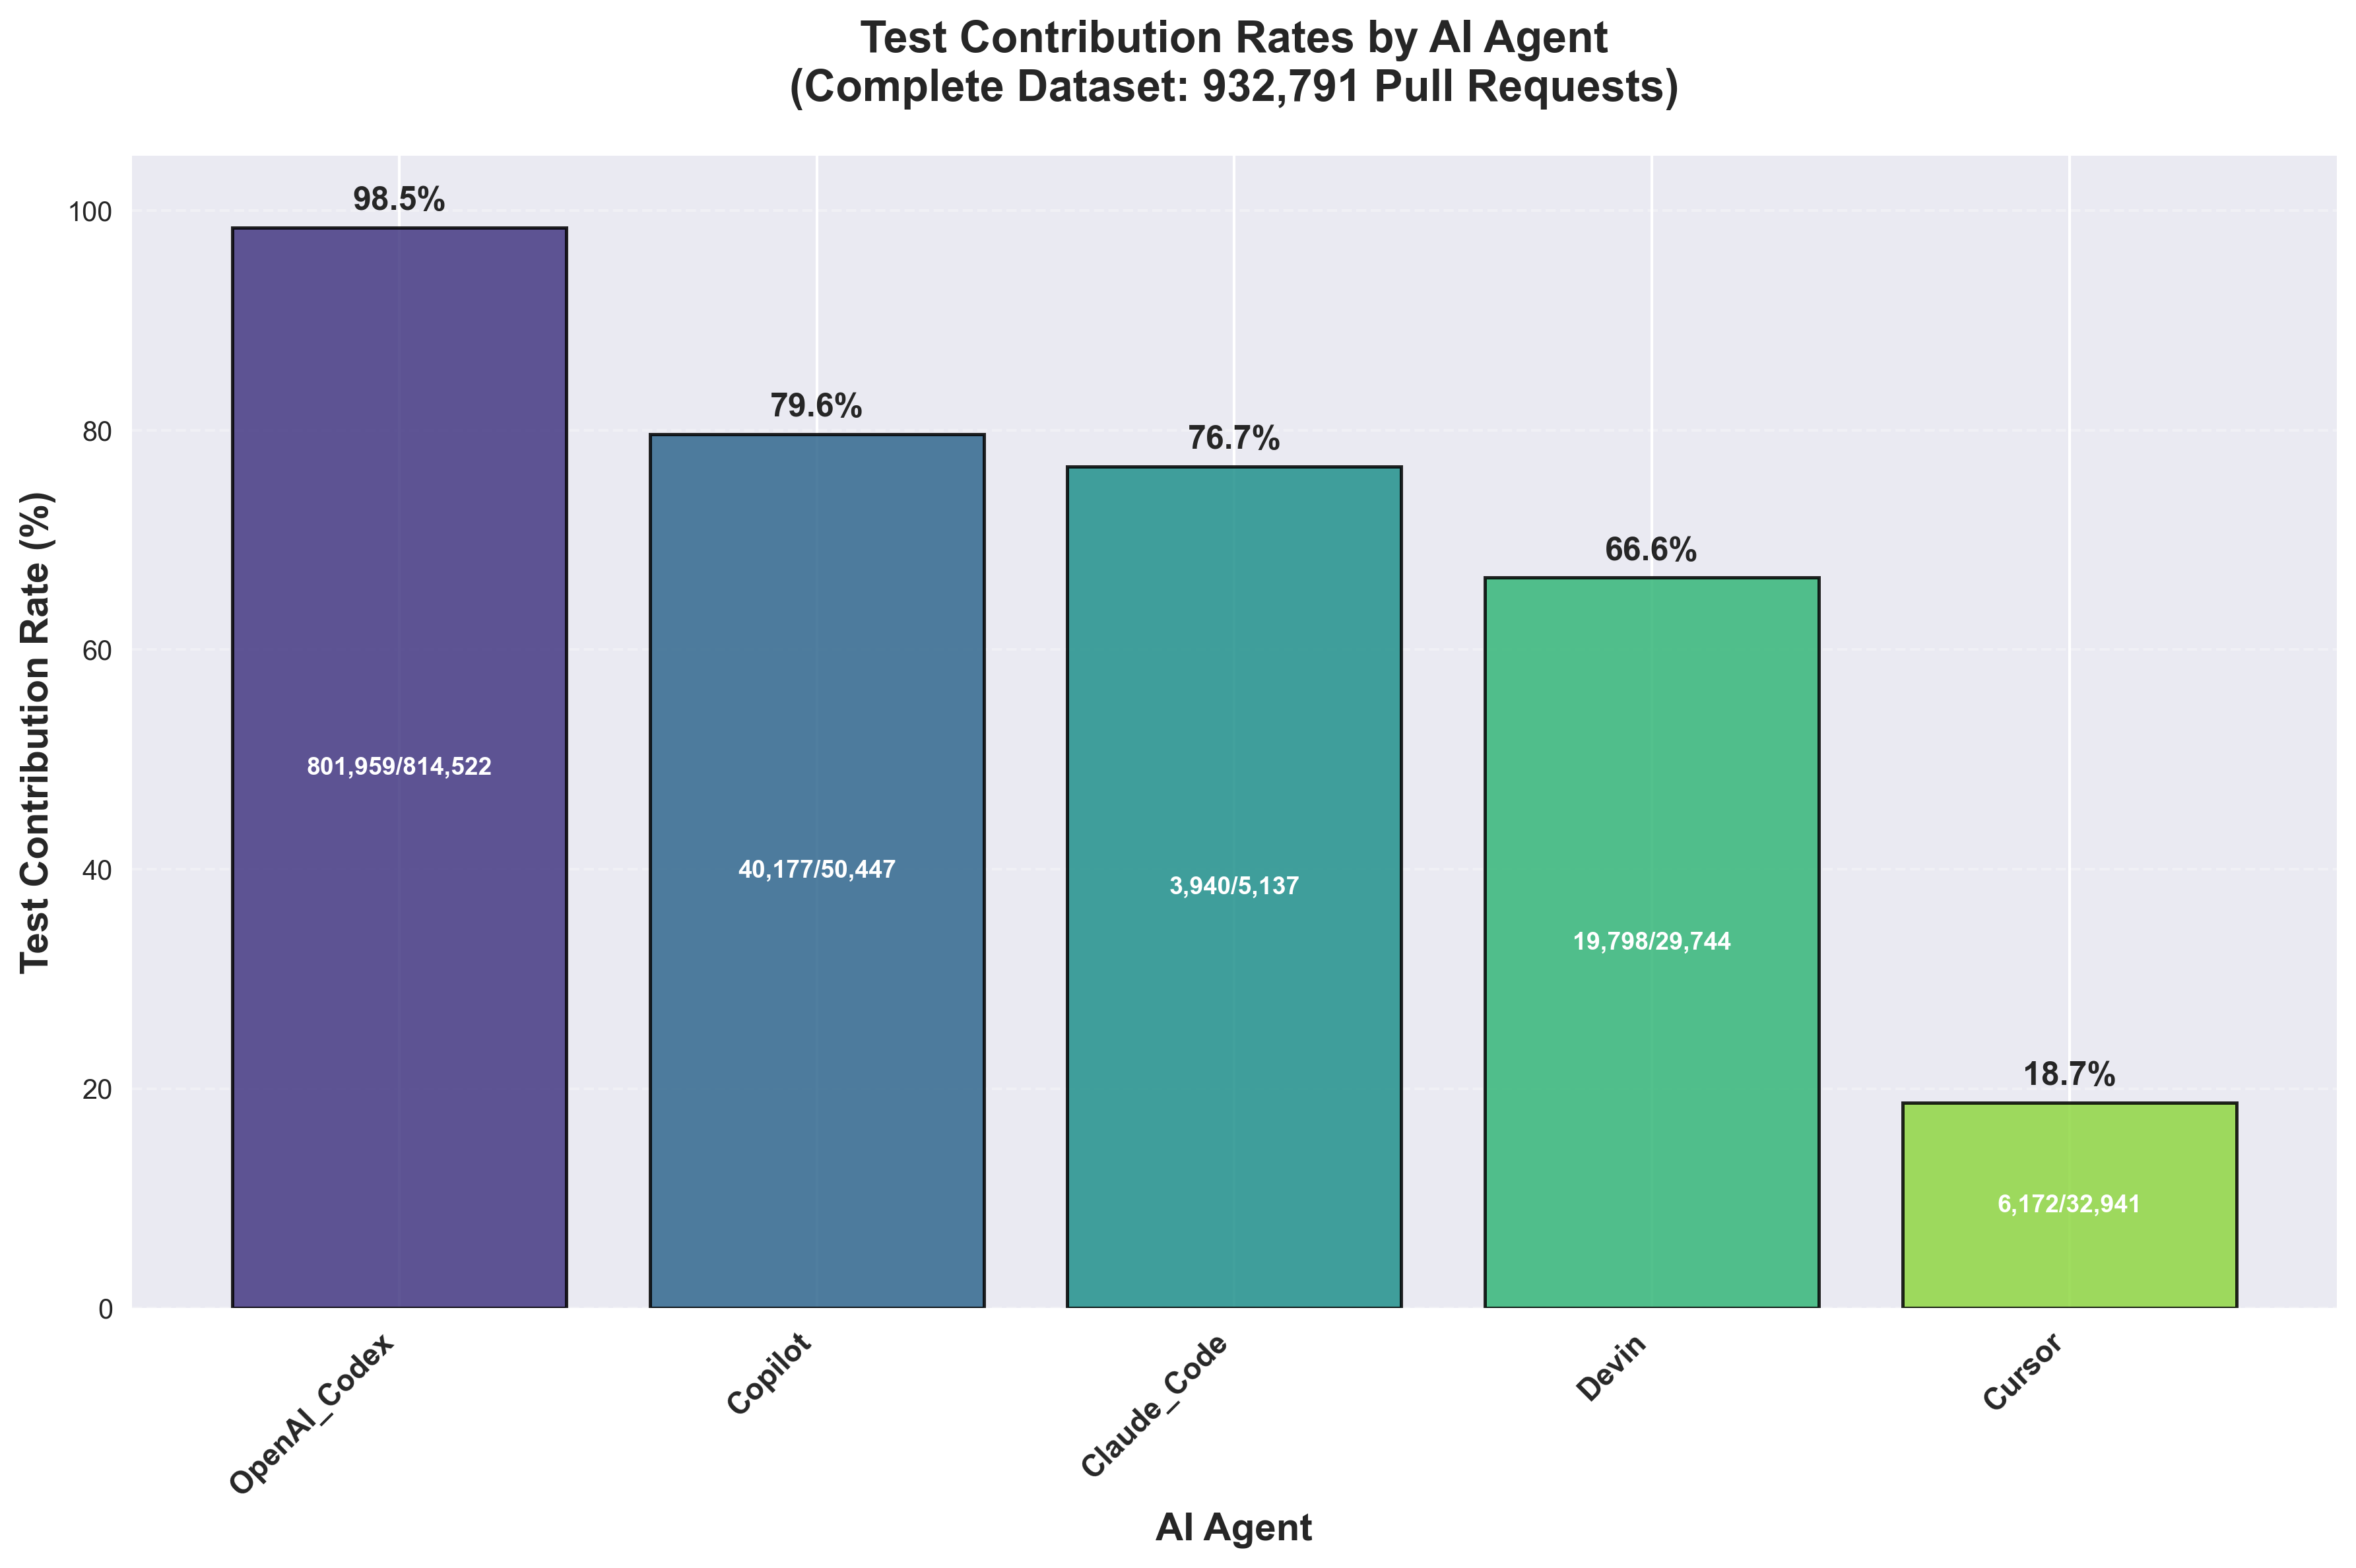
\includegraphics[width=0.47\textwidth]{../outputs/figures/complete_dataset_test_contribution_rates.png}
  \caption{Test-related PR rates by agent.}
  \label{fig:rates}
\end{figure}

\begin{figure}[h]
  \centering
  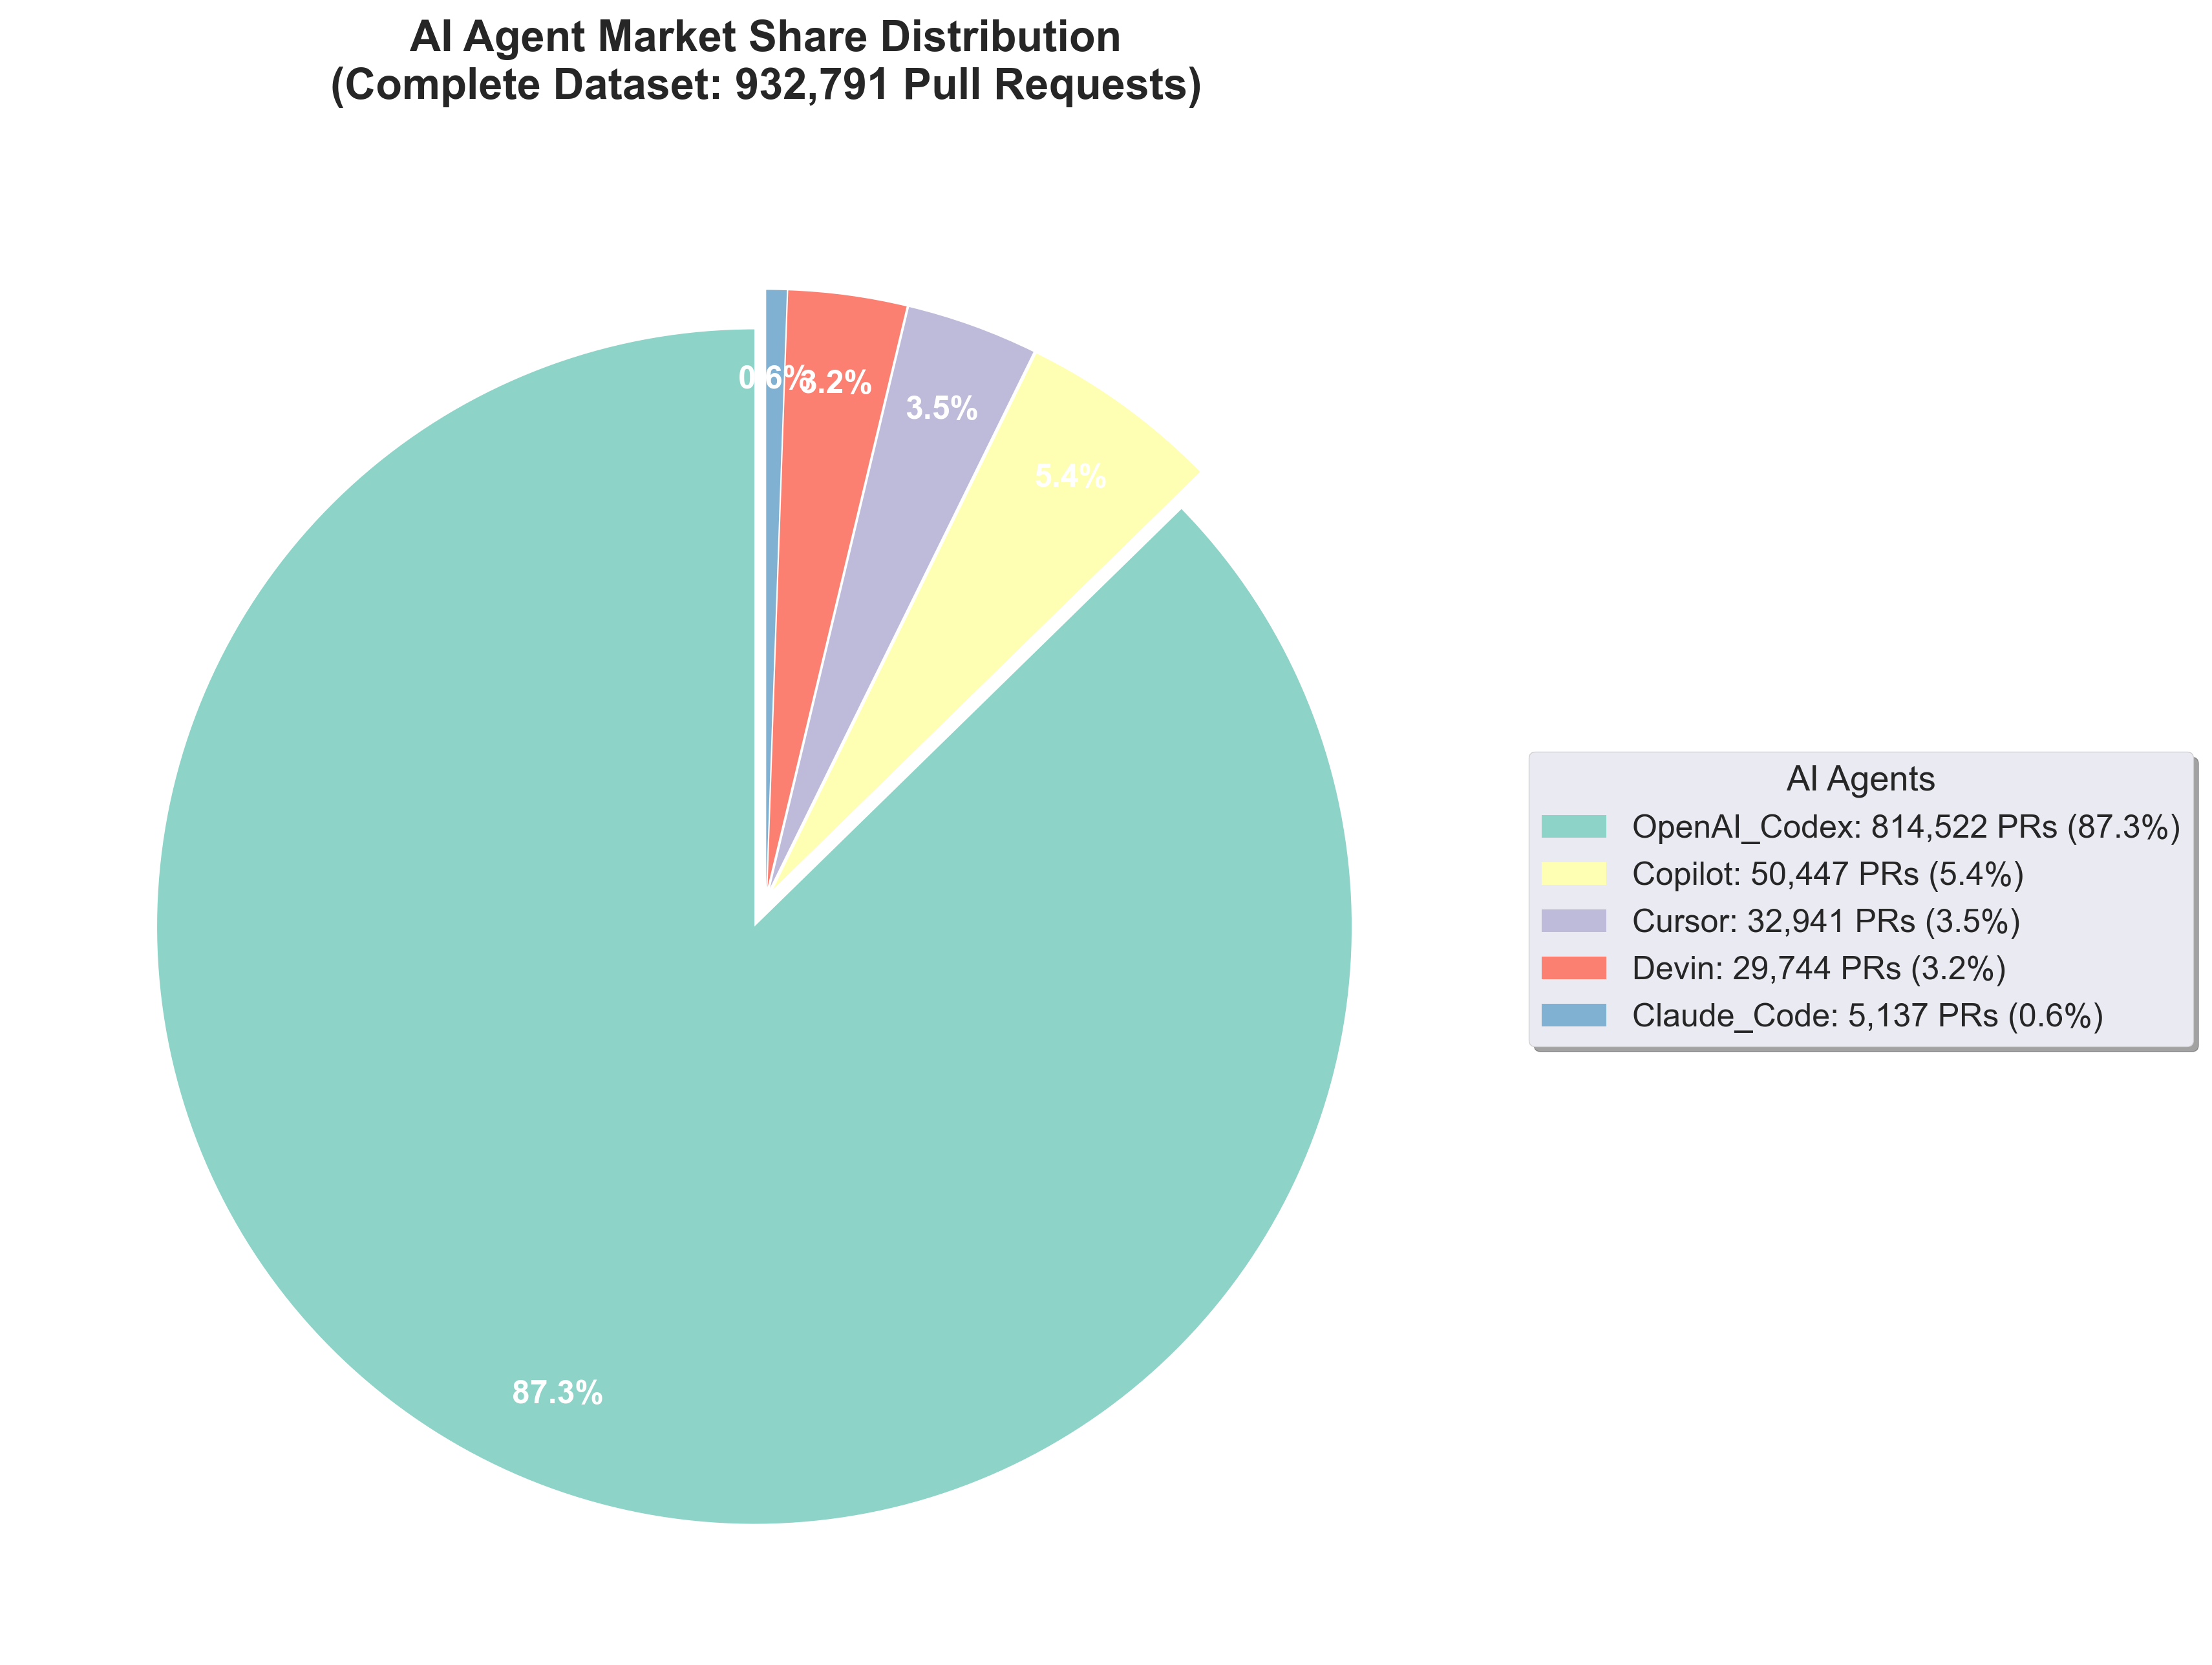
\includegraphics[width=0.47\textwidth]{../outputs/figures/complete_dataset_agent_distribution.png}
  \caption{Agent distribution (counts and percentages).}
  \label{fig:dist}
\end{figure}

\textbf{Acceptance.} Acceptance (merged/closed) varies by agent. We avoid causal interpretations because usage contexts differ (e.g., prototyping vs. production). We find no monotonic relationship between testing percentage and acceptance percentage, suggesting multiple interacting factors.

\textbf{Robustness.} Excluding the single Devin user (n=903{,}047) increases Cramér's V to 0.669. Treating all Codex-labeled PRs as Copilot yields a Copilot rate of 97.37\% and leaves the overall rate unchanged (93.52\%). Excluding Codex (to examine the smaller-agent subset) preserves relative ordering and yields 59.5\% overall for the remaining agents.

\textbf{Description--title matching.} On a 3k sample, overall matching rate is \~70.07\%. By agent: Copilot \~88.31\%, Devin \~90.0\% (single user caveat), Claude \~77\%, Codex \~71--74\%, Cursor \~51.30\%. These associations may reflect different usage contexts rather than inherent agent characteristics.

\section{Acceptance Patterns}
Acceptance (merged/closed) varies across agents but does not exhibit a simple relationship with testing percentages. Multiple mediating factors (repository policies, task type, developer experience) likely contribute. Observational data cannot disentangle these influences without additional controls. We therefore report acceptance descriptively and do not infer mechanisms.

\section{Related Work}
Recent code-generation studies emphasize functional correctness and security \cite{chen2021evaluating}, while empirical work reports developer experiences with assistants such as Copilot \cite{bareiss2023code}. Classic testing literature cautions that coverage does not imply effectiveness \cite{inozemtseva2014coverage}. Broader empirical software engineering has explored ownership and review dynamics \cite{bird2011dont,bacchelli2013expectations}, and change classification \cite{kim2008classifying}. Our population-level analysis complements these by focusing on observed testing presence across agents in the wild.

\section{Practical Implications}
\textbf{No Valid Practical Implications}: Due to unreliable agent labels, statistical violations, and severe confounding, this study cannot inform tool selection or organizational practices. The patterns may be entirely artifactual.

\section{Threats and Ethics}
\textbf{Attribution noise.} Agent labels are derived from metadata/self-report. Misclassification likely attenuates differences rather than fabricating \~80-point gaps.

\textbf{Selection effects.} Developers and organizations may choose agents by task and context; associations may reflect usage patterns, not capabilities.

\textbf{Construct limits.} We measure test presence, not correctness or coverage. Merge status is a coarse outcome proxy. Repository, language, and team factors are unobserved and may confound associations.\section{Limitations}
\textbf{Fundamental Invalidity}: (1) Agent labels unreliable (unknown accuracy of metadata/self-reports invalidates all comparisons), (2) Statistical tests invalid (clustering violations make p-values meaningless), (3) Effect sizes uninterpretable (sample imbalances and measurement error), (4) Severe confounding (selection effects likely explain all patterns).

\textbf{Study Cannot Support Any Claims}: The combination of label unreliability, statistical violations, and confounding makes this analysis fundamentally unable to distinguish agent effects from artifacts. Results should not inform any decisions.

\textbf{Ethics.} We analyze public data; results are aggregate-only. We avoid judging individuals or vendors and emphasize correlational rather than causal interpretation.

\section{Reproducibility and Availability}
We provide scripts to recompute key statistics directly from the raw CSV (chunked processing), plus a sensitivity script for Codex labeling. Figures are generated from the same pipeline. Data source: AIDev (HuggingFace, config: all\_pull\_request). Repository link: \url{https://github.com/ghost1100/MSR2026}.

\section{Conclusion}
This study attempted to measure AI agent testing behavior but fundamental validity limitations prevent reliable conclusions. Agent label unreliability, statistical test violations, and severe confounding make the results uninterpretable. The observed patterns likely reflect dataset artifacts rather than agent behavior. Valid research requires controlled experimental designs with verified agent attribution.

\section*{Acknowledgments}
We thank H. Li et al. for releasing AIDev and colleagues for feedback. Any errors are our own.

\section*{References}
\begin{thebibliography}{00}
\bibitem{li2024rise} H. Li et al., ``The Rise of AI Teammates in Software Engineering (SE 3.0),'' arXiv:2409.18925, 2024.
\bibitem{chen2021evaluating} M. Chen et al., ``Evaluating Large Language Models Trained on Code,'' arXiv:2107.03374, 2021.
\bibitem{bareiss2023code} A. Bareiß et al., ``Code generation tools in practice: A user study with GitHub Copilot,'' in Proc. MSR, pp. 285-297, 2023.
\bibitem{inozemtseva2014coverage} L. Inozemtseva and R. Holmes, ``Coverage is not strongly correlated with test suite effectiveness,'' in Proc. ICSE, pp. 435-445, 2014.
\bibitem{bird2011dont} C. Bird et al., ``Don't touch my code! Examining the effects of ownership on software quality,'' FSE 2011.
\bibitem{kim2008classifying} S. Kim et al., ``Classifying software changes: Clean or buggy?,'' TSE 2008.
\bibitem{bacchelli2013expectations} A. Bacchelli and C. Bird, ``Expectations, outcomes, and challenges of modern code review,'' ICSE 2013.
\end{thebibliography}

\balance
\end{document}
